\documentclass{article}%
\usepackage[T1]{fontenc}%
\usepackage[utf8]{inputenc}%
\usepackage{lmodern}%
\usepackage{textcomp}%
\usepackage{lastpage}%
\usepackage[head=40pt,margin=0.5in,bottom=0.6in]{geometry}%
\usepackage{graphicx}%
%
\title{\textbf{Rechazaron plan estatal para formar profesores}}%
\author{El Nacional}%
\date{17/10/2018}%
%
\begin{document}%
\normalsize%
\maketitle%
\textbf{URL: }%
http://www.el{-}nacional.com/noticias/educacion/rechazaron{-}plan{-}estatal{-}para{-}formar{-}profesores\_256061\newline%
%
\textbf{Periodico: }%
EN, %
ID: %
256061, %
Seccion: %
Educación\newline%
%
\textbf{Palabras Claves: }%
NO\_TIENE\newline%
%
\textbf{Derecho: }%
2.2%
, Otros Derechos: %
NO\_TIENE%
, Sub Derechos: %
2.2.1%
\newline%
%
\textbf{EP: }%
NO\newline%
\newline%
%
\textbf{\textit{El presidente Nicolás Maduro declaró convertir la micromisión Simón Rodríguez en la Universidad Nacional Experimental del Magisterio Venezolano Samuel Robinson}}%
\newline%
\newline%
%
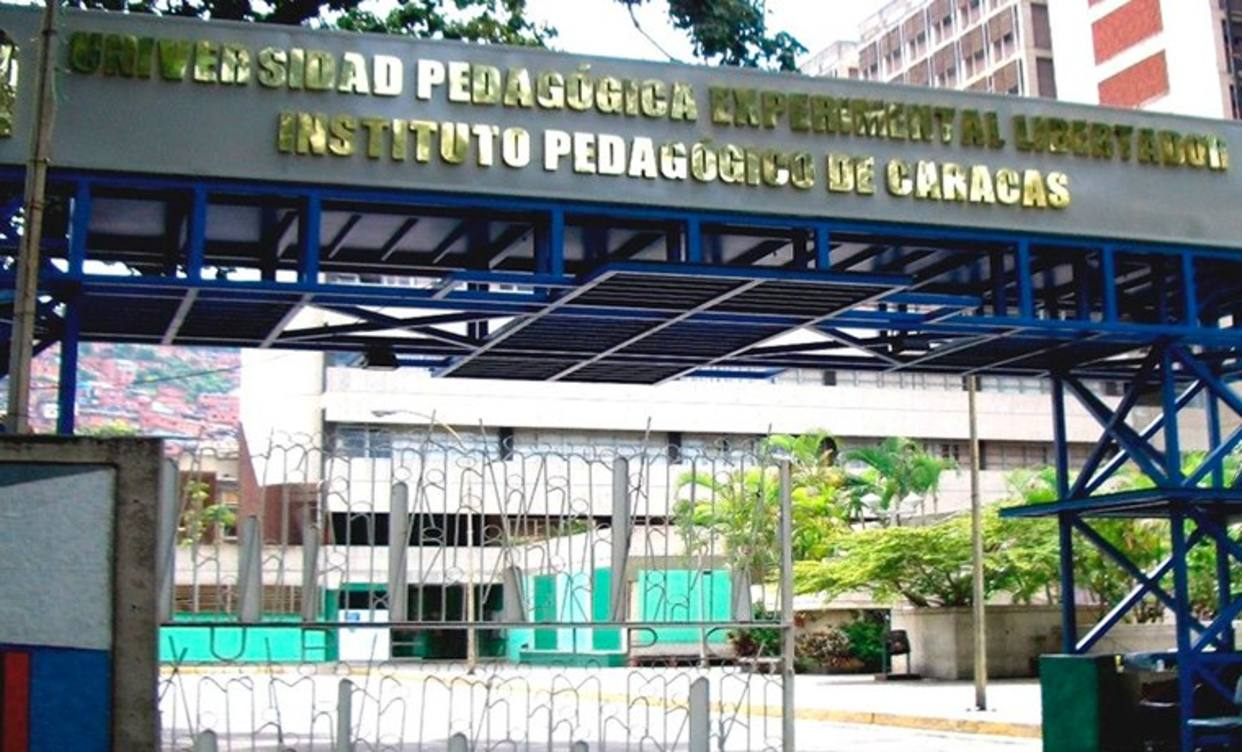
\includegraphics[width=300px]{156.jpg}%
\newline%
%
Luego del anuncio del 18 de septiembre según el cual el presidente Nicolás Maduro declaró convertir la micromisión Simón Rodríguez en la Universidad Nacional Experimental del Magisterio Venezolano Samuel Robinson,~el rector de la Universidad Pedagógica Experimental Libertador, Raúl López Sayago,~expresó su rechazo a través de una nota de prensa en la que considera que la institución encargada de formar a los docentes es por excelencia la UPEL.%
\newline%
%
Sayago declaró que esta institución, que cuenta con más de 82 años de trayectoria, está al servicio del país y que ha cumplido con la necesidad y el propósito de formar docentes de altísima calidad.%
\newline%
%
El rector hizo un llamado a trabajar de manera conjunta en cualquier proyecto que proponga el Estado venezolano,“siempre que esa formación esté en correspondencia con los principios de autonomía, democracia, pluralidad y de formar docentes al servicio del país”.%
\newline%
%
Manifestó que el gobierno debería invertir para mejorar su infraestructura física y funcional en las universidades que ya existen, pues dijo no entender por qué piensan en crear una nueva universidad, cuando tanto la UPEL como el resto de las casas de estudios superiores cuentan con la capacidad para atender esta demanda.%
\newline%
%
\end{document}